% Author: Abid H. Mujtaba

% This is a tex file implementing my CV/resume.

\documentclass[11pt]{article}


% Configuration copied from source tex file mentioned in webpage: http://www.thelinuxdaily.com/2008/10/latex-resume-examples/  by Derek R. Hildreth

\usepackage{latexsym}
\usepackage[empty]{fullpage}
\usepackage[usenames,dvipsnames]{xcolor}
\usepackage{verbatim}
\usepackage[pdftex]{hyperref}

\usepackage{graphicx}
\usepackage{setspace}
\usepackage{changepage}

\hypersetup{
	colorlinks,
	citecolor=black,
	filecolor=black,
	linkcolor=black,
	urlcolor=mygreylink
}

\urlstyle{same}
\definecolor{mygrey}{gray}{.85}
\definecolor{mygreylink}{gray}{.10}
\textheight=9.0in
\raggedbottom
\raggedright
\setlength{\tabcolsep}{0in}

% Adjust margins
\addtolength{\oddsidemargin}{-0.375in}
\addtolength{\evensidemargin}{0.375in}
\addtolength{\textwidth}{0.5in}
\addtolength{\topmargin}{-.375in}
\addtolength{\textheight}{0.75in}

%-----------------------------------------------------------
%Custom commands
\newcommand{\resitem}[1]{\item #1 \vspace{-2pt}}
\newcommand{\resheading}[1]{{\large \colorbox{mygrey}{\begin{minipage}{\textwidth}{\textbf{#1 \vphantom{p\^{E}}}}\end{minipage}}}}
\newcommand{\ressubheading}[4]{
\begin{tabular*}{6.5in}{l@{\extracolsep{\fill}}r}
		\textbf{#1} & #2 \\
		\textit{#3} & \textit{#4} \\
\end{tabular*}\vspace{-6pt}}


\usepackage{array, xcolor}			% Settings from http://texblog.org/2012/04/25/writing-a-cv-in-latex/
\definecolor{lightgray}{gray}{0.8}

\newcommand\VRule{\color{lightgray}\vrule width 0.5pt}

\usepackage{hanging}

% New Environments:


\newenvironment{hindent}{\hspace{30pt}\begin{minipage}{0.9\textwidth}}{\end{minipage}}		% Hanging Indentation used for text inside each section

\newenvironment{Section}[1]{\resheading{#1}\vspace{10pt}}{\vspace{12pt}}		% A Section environment that accepts the heading of the section as the parameter

\newenvironment{nbList}{\vspace{-10pt}\renewcommand\labelitemi{}\begin{itemize}}{\end{itemize}\vspace{-10pt}}		% A List environment with no bullets.

\newenvironment{specTable}[1]{\begin{tabular}{l@{ : }p{#1\textwidth}}}{\end{tabular}}		% Specifies a 2-column table separated by a colon used to specify items. The second column has wrapped text

\newcommand\twoTable[3]{\begin{tabular}{p{0.12\textwidth}@{ - \hspace{0.5em}}p{0.12\textwidth}@{\hspace{2em}}p{0.6\textwidth}}#1 & #2 & #3 \end{tabular}}


\DeclareGraphicsExtensions{.jpg}

%%%%%%%%%%%%%%%%%%%%%%%%%%%%%%%%%%%%%%%%%%%%%5





\begin{document}

%%%%% First we construct the top section containing the name, address and photograph

% Insert portrait
\begin{flushright}
	\makebox[0pt][r]{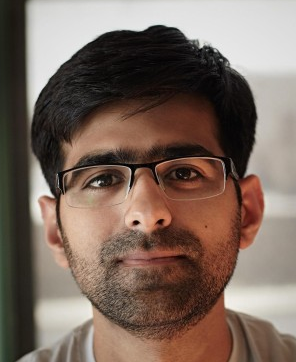
\includegraphics[width=0.15\linewidth]{portrait.png}}
\end{flushright}
%
\begin{center}

	\vspace{-9\baselineskip}
	\textbf{\Huge \textcolor{mygreylink}{Abid Hasan Mujtaba}}
	\vspace{16pt}

	\begin{onehalfspace}
	{\large
		192 Mill Road, Valley Stream, NY-11581

		\vspace{4pt}
		914-309-6003

		\href{mailto:abid.naqvi83@gmail.com}{abid.naqvi83@gmail.com}
	}
	\end{onehalfspace}
	\vspace{2\baselineskip}

\end{center}


%%%%%


\begin{Section}{Objective}

	\begin{hindent}

		Seeking a challenging position as a Software Engineering Trainer

	\end{hindent}

\end{Section}



\begin{Section}{Nationality}

	\begin{hindent}

		U.S. Citizen

	\end{hindent}

\end{Section}



\begin{Section}{Education}

	\vspace{-10pt}
	\begin{doublespace}

		\begin{tabular}{>{\raggedleft}p{0.1\textwidth}@{  --  }p{0.07\textwidth}@{\hspace{15pt}}p{0.7\textwidth}}
			2006 & 2012 & {\bf PhD in Theoretical Physics}, Texas A\&M University \\
			2002 & 2006  & BE in Electrical Engineering, EME College, NUST, Pakistan \\
		\end{tabular}

	\end{doublespace}
	\vspace{-10pt}

\end{Section}


\begin{Section}{Experience}

	\begin{nbList}
		\item \twoTable{Jan. 2021}{}{\textbf{Software Engineering Trainer}, Continuing Education, Bloomberg LP}

			\begin{adjustwidth}{4em}{}
				Create and offer trainings to all Engineers on advanced (Advanced topics in Python, Messaging \& Distributed Systems, Operational Resilience, S3, etc.) and new (MCP Servers, Argo Workflows, IAM, etc.) topics.

				Create and maintain tooling for the automated generation of training materials and labs.
			\end{adjustwidth}

		\item \twoTable{Oct. 2018}{Dec. 2021}{\textbf{Software Engineering Trainer}, Entry-Level Training, Bloomberg LP}

			\begin{adjustwidth}{4em}{}
				Onboard college graduates (both CS and non-CS) into Bloomberg Engineering, covering Python and Typescript,
				and Bloomberg's internal 3-tier stack as well as local development, testing, and deployment
			\end{adjustwidth}

		\item \twoTable{Mar. 2015}{Jul. 2018}{\textbf{Assistant Professor}, COMSATS University Islamabad.}

			\begin{adjustwidth}{4em}{}
				Focus on Mathematical and Computational Physics. Carrying out research in pedagogy (using R for data analysis), General Relativity (Python and Cython), Numerical Plasma Physics (C and R), and the Foundations of Quantum Mechanics.
			\end{adjustwidth}

		\item \twoTable{Oct. 2013}{Mar. 2016}{\textbf{Android/Python Developer}, SpotOn Inc., Chicago.}

			\begin{adjustwidth}{4em}{}
				Tasked with, initially individually and later as team leader, \
				creating and maintaining native Android applications \
				(from scratch, based on designs and requirements) for both \
				clients (100,000s) and merchants (1000s) signed up with \
				SpotOn's digital loyalty program.
			\end{adjustwidth}

		\item \twoTable{Feb. 2013}{Oct. 2013}{\textbf{Python Developer}, Sanders New Media, Chicago.}

			\begin{adjustwidth}{4em}{}
				Developing Python front and back-end solutions for various clients including Django-based CMS websites, Selenium-based testing, and ZeroMQ-based load-balancers.
			\end{adjustwidth}

	\end{nbList}

\end{Section}



\begin{Section}{Technical Skills}

	\begin{nbList}

		\item \textbf{Languages} : Python, Typescript, C++, C, Cython, Java, Haskell, Lua, Bash, PHP, Visual Basic

		\item \textbf{Operating Systems} : Arch Linux, Ubuntu, Mac OS X, MS Windows

		\item \textbf{AI} : Claude Code (including the SDK), Github Copilot, ChatGPT

		\item \textbf{Computational Software} : R, Sage, Matlab, Mathematica

		\item \textbf{Markup Languages} : (X)HTML, CSS, XML, \LaTeX

		\item \textbf{Servers \& DBMS} : Apache and Nginx (Python (Django) and PHP cgi scripting), MySQL, PostgreSQL, MongoDB

		\item \textbf{Miscellaneous} : Git, make, ZeroMQ (Messaging), Gimp \& Inkscape (Graphics)

	\end{nbList}

\end{Section}


\begin{Section}{Online Presence}

    \begin{nbList}

    	\item \textbf{Open Source Projects} : \href{https://github.com/abid-mujtaba}{github.com/abid-mujtaba}

    	\item \textbf{Technical Blog} : \href{https://abidmujtaba.blogspot.com}{abidmujtaba.blogspot.com}

    	\item \textbf{Professional Network} : \href{https://linkedin.com/in/abid-mujtaba-2696a5163}{linkedin.com/in/abid-mujtaba-2696a5163}

		\item \textbf{Academic Research} : \href{https://researchgate.net/profile/Abid-Mujtaba}{researchgate.net/profile/Abid-Mujtaba}

    \end{nbList}

\end{Section}


\begin{Section}{Relevant Coursework}

	\begin{nbList}

		\item \begin{specTable}{0.9}\textbf{UG} & Algorithms \& Computing (\textit{C++}), Data Structures (\textit{C++}), Signals Systems \& Filters (\textit{Matlab}), Digital Signal Processing \& Filter Design (\textit{Matlab}), Fuzzy Logic \& Neural Network\end{specTable}

		\item \begin{specTable}{0.9}\textbf{PG} & Computational Physics, Quantum Computing \end{specTable}


	\end{nbList}

\end{Section}

\end{document}
